\chapter{Das Referenzmodell: Einzelne Kugel auf festem Grund}



\section{Erstellung und Equilibrierung der Probe}
	Eine Probe im Sinne der MD ist eine Datei, welche mindestens alle notwendigen Eigenschaften
	aller Teilchen im System speichert. Dazu gehören natürlich der Ort und die Geschwindigkeit
	jedes Teilchens, aber auch der Teilchentyp und die Teilchenmasse. Der Mulde im LJ-Potential
	\eqref{eq:potential_lj} nach gibt es für alle Teilchen einen Zustand minimaler Energie.
	Aus diesem Grund existiert ein stationärer Gleichgewichtzustand (\emph{Equilibrium}). Den
	Gesetzen der Thermodynamik folgend geht jedes ungestörte Nichtgleichgewichtssystem in sein
	Equilibrium über. Dieser Vorgang heißt \emph{Equilibrierung}. Da eine Probe prinzipiell einen
	beliebigen Zustand haben kann, ist eine \emph{vorherige} Equilibrierung besonders wichtig.
	Andernfalls findet der Equilibrierungsprozess gestört während der eigentlichen Simulation
	statt, was zu verfälschten Ergebnissen führen kann.

	Für das Modell dieser Arbeit bietet es sich an, eine auf \SI{300}{\kelvin} aufgeheizte Probe
	zu betrachten. Viele der in der Literatur auffindbaren Vergleichswerte zu Materialkonstanten
	werden bei diesem der Raumtemperatur nahe gelegenen Wert angegeben. Zudem bildet diese
	Temperatur das Problem gut ab.

	\subsection{Homogene Deformation}
		Um eine Probe nun in ihren Gleichgewichtszustand mit dieser Temperatur zu versetzen bietet
		es sich an, zuerst eine Probe der Temperatur \SI{0}{\kelvin} zu erstellen und diese dann
		aufzuheizen. Der rechnerische Nullpunkt lässt sich einfach dadurch erreichen, dass die
		Teilchengeschwindigkeiten auf 0 gesetzt werden. Mithilfe einer homogenen Deformation wird
		eine Simulation ohne Berücksichtigung der durch die Kraft verursachten Teilchenbewegungen
		durchgeführt. In jedem Simulationsschritt wird die Probe mithilfe einer zum Gitter
		achsenparallel wirkenden Deformationsmatrix inkrementell skaliert. Der sich dadurch
		ergebende Verlauf der mittleren potentiellen Energie kann nun minimiert werden. Aufgrund
		der Proportionalität zwischen dem Druck und den gemittelten Kräften äußert sich diese
		Stelle in Abbildung \ref{fig:homdef} in Form einer Nullstelle genau dort, wo die
		potentielle Energie minimal ist. Dies ist auch in sofern einleuchtend, da der Druck
		angibt, inwiefern sich einen Probe beim loslassen zusammenziehen oder ausdehnen würde
		\cite{rapp2014laserablation}.

		\begin{figure}[!ht]
			\centering
			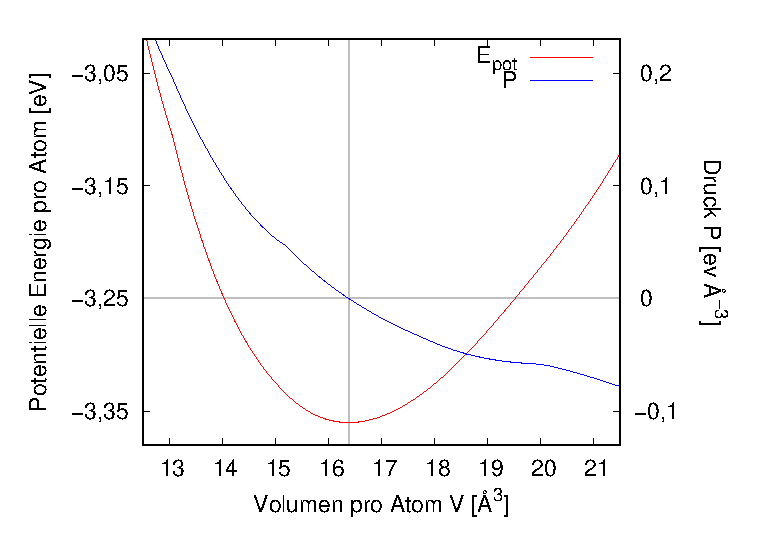
\includegraphics[width=0.9\textwidth]{chapter/main/single/plt/equilibration/homdef.eps}
			\caption{Die mittlere potentielle Energie und der Probendruck aufgetragen gegen das
			Volumen pro Teilchen. Das Energieminimum kann durch einen näherungsweise quadratischen
			Fit um das Minimum der potentiellen Energie oder über eine Nullstellensuche des Druck
			bestimmt werden. In diesem Fall liegt das Energieminimum bei einem Teilchenvolumen von
			\SI{16.38}{\angstrom\cubed}.}
			\label{fig:homdef}
		\end{figure}

	\subsection{Aufheizen der Probe}
		Die bisherige Simulation fand unter Beachtung der Regeln eines mikrokanonischen Ensembles
		(\emph{NVE}) statt. Das bedeutet, dass neben der Teilchenzahl $N$ und dem Volumen $V$ die
		Gesamtenergie $E$ festgehalten wurde. Da im nächsten Schritt eine Temperaturerhöhung zum
		Aufheizen der Probe notwendig ist, ist ein NVE-Ensemble System so zwangsläufig ungeeignet.
		Stattdessen bietet sich das kanonische Ensemble (\emph{NVT}) an. Hier werden auch die
		Teilchenzahl und das Volumen fest gesetzt, allerdings wird hier statt der Energie die
		Temperatur $T$ durch Kopplung an ein Wärmebad vorgegeben. In der Simulation wird dies
		mithilfe eines Thermostats realisiert. Ein Thermostat manipuliert dabei die Simulation in
		der Hinsicht, dass die Temperatur der Vorgabe entspricht. Ein einfacher Thermostat wäre
		das Berendsen-Thermostat, bei dem der durch das Äquipartitionstheorem
		\eqref{eq:equipartition} gegebene Zusammenhang zwischen Temperatur und
		Teilchengeschwindigkeit genutzt wird, um alle Teilchengeschwindigkeiten global zu
		reskalieren. Dies hat allerdings einen Verlust der Maxwell-Boltzmann-Verteilung der
		Geschwindigkeitsbeträge zur Folge. Der in IMD verwendete Thermostat ist deshalb das
		\emph{Nosé-Hoover-Thermostat} \cite{rapp2014laserablation}.

		\begin{figure}[!ht]
			\centering
			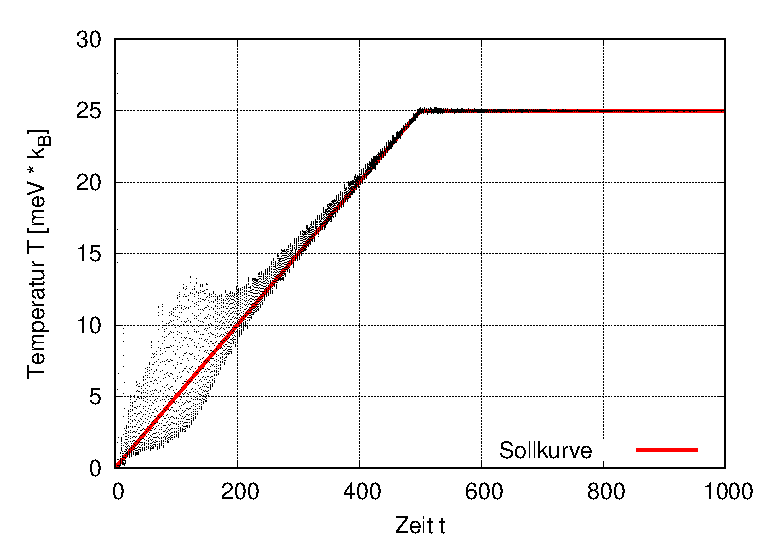
\includegraphics[width=0.9\textwidth]{chapter/main/single/plt/equilibration/thermostat.eps}
			\caption{Der Aufheizprozess mit vorgegebener Temperatur. Die Fluktuationen werden
			mit fortschreitender Zeit geringer.}
			\label{fig:thermostat}
		\end{figure}

		Abbildung \ref{fig:thermostat} zeigt das Aufheizen einer würfelförmigen Probe mithilfe des
		in IMD implementierten Nosé-Hoover-Thermostats. Während die Temperatur am Anfang trotz
		Vorgabe noch schwankt, vermindert sich dieser Effekt mit der Zeit. Ab ungefähr 800
		IMD-Zeiteinheiten sind die Fluktuationen in etwa konstant.

		\begin{figure}[!ht]
			\centering
			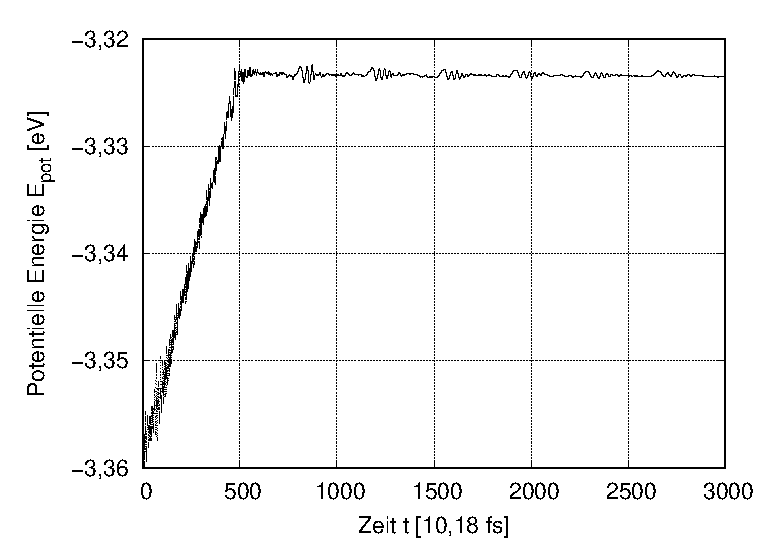
\includegraphics[width=0.9\textwidth]{chapter/main/single/plt/equilibration/thermostat_pot.eps}
			\caption{Die potentielle Energie zeigt einen zur Temperatur proportionalen Verlauf}
			\label{fig:thermostat_pot}
		\end{figure}

		Wie allerdings in Abbildung \ref{fig:thermostat_pot} zu sehen ist, verhält sich die
		potentielle Energie proportional zum Temperaturverlauf. Von daher ist es ratsam nach dem
		Aufheizen eine NVE-Simulation bis zum Equilibrium durchzuführen.

	\subsection{Erzeugen einer Kugelprobe}
		Üblicherweise sind Proben quaderförmig und bilden durch \emph{periodischen Randbedingungen}
		(\emph{PBC}) ein Gitter, welches teilweise Eigenschaften eines unendlich ausgedehnten
		Gitters imitiert. Im Rahmen dieser Arbeit sind jedoch Kugelformen unter der Einwirkung von
		Gravitation interessant, da sie so den Pulverpartikeln beim SLM-Verfahren sehr ähnlich
		sind. Die einfachste Methode zum Erzeugen einer solchen Probe ist die Wahl eines
		entsprechenden Gitterausschnitts, wobei die umliegenden Teilchen entfernt werden.
		Hierbei gilt zu beachten, dass die Kugel erst nach der homogenen Deformation freigestellt
		wird. Das hat den Grund, dass eine homogene Deformation das gesamte Teilchensystem
		skaliert. Ist der Radius der Kugel sehr genau bemaßt, ändert er sich signifikant während
		dieses Prozesses. Wichtig ist für die nachfolgenden Equilibrierungsschritte auf jeden
		Fall, dass diese nun unter Einfluss der Gravitation mit ausreichend Equilibrierungszeit
		erfolgen. So wird gewährleistet, dass die Kugel etwas absackt und sich somit in ihre der
		Form entsprechenden Ruhelage begibt. Abbildung \ref{fig:equilibrated_sample} zeigt dabei
		die Ruhelage eines kugelförmigen Gitterausschnitts mit einem Durchmesser von
		\SI{400}{\angstrom}. Zwischen fixiertem Boden und beweglicher Kugel vergrößert sich die
		Kontaktfläche durch die Wirkung der Gravitation.

		Es ist allgemein empfehlenswert, wenn die Kugel nicht direkt in den Einflussbereich der
		PBC positioniert wird. Um eine derartige Selbstbeeinflussung zu verhindern könnten die PBC
		deaktiviert werden, jedoch stellten diese sich für die Erstellung problemverwandter Proben
		als nützlich heraus. So kann beispielsweise eine Simulationsbox mehrfach
		hintereinanderkopiert werden, um eine Reihe an Kugeln zu erhalten. Sofern diese
		ursprüngliche Probe mit PBC equilibriert wurde, sind randübergreifende Aspekte wie der
		Boden nahtlos wiederholbar, wodurch das System nicht erneut equilibriert werden muss. Das
		spart vor allem bei größeren Proben Zeit.

		\begin{figure}[!ht]
			\centering
			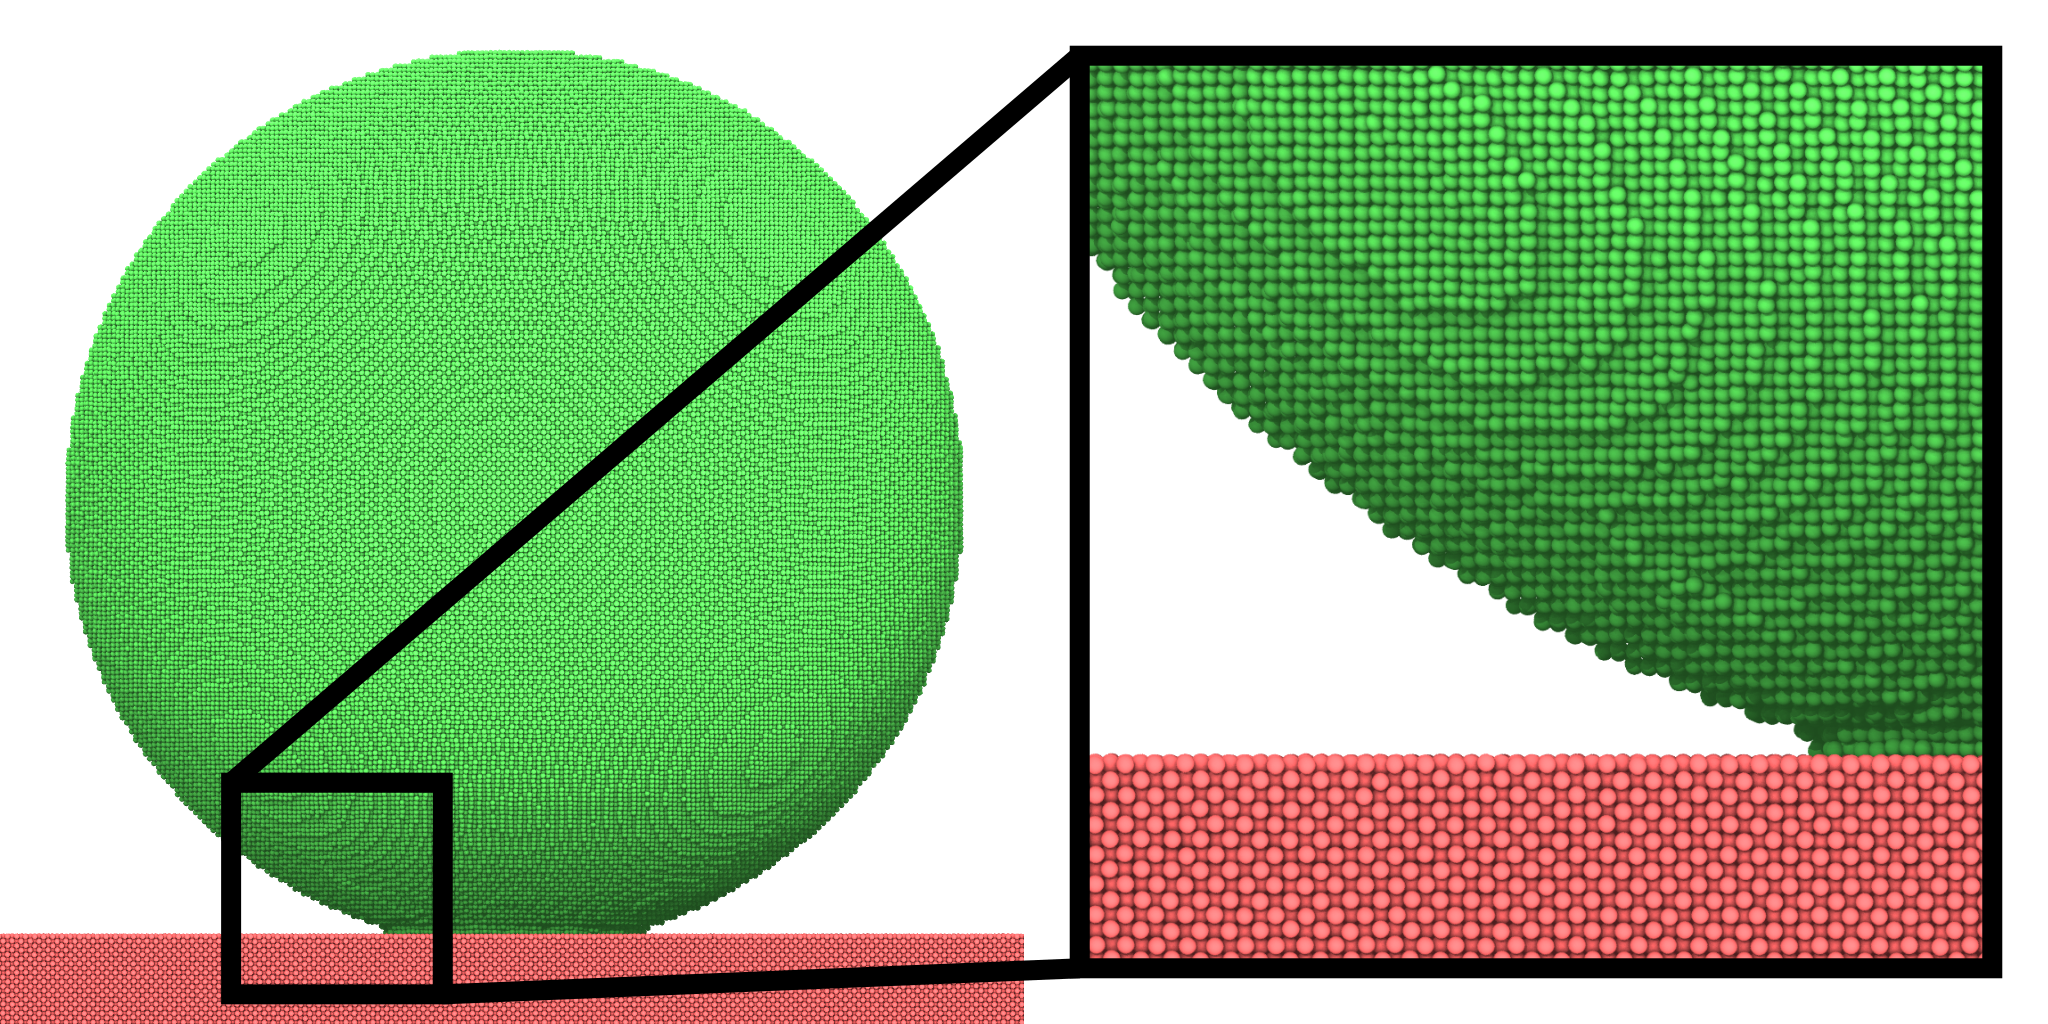
\includegraphics[width=\textwidth]{chapter/main/single/img/equilibrated_sphere.zoom.png}
			\caption{Eine vollständig equilibrierte Kugel aus Aluminiumatomen (grün) auf einem
			festen, unbeweglichen Untergrund (rot) vergrößert die Kontaktfläche unter dem eigenen
			Gewicht}
			\label{fig:equilibrated_sample}
		\end{figure}


\section{Variation der Laserleistung bei fester Lasergeschwindigkeit}
		Wie in Abschnitt \ref{subsec:approximation} bereits erläutert werden für dieses Modell
		teils Näherungen verwendet, die ein direktes Übertragen der Simulationsdaten auf
		experimentelle Messdaten anhand einer reinen Messgrößenumrechnung nahezu unmöglich machen.
		Zur Verifizierung des Modells bietet sich also ein überwiegend qualitativer Vergleich mit
		Beobachtungen aus Experimenten an.

		\begin{figure}[!ht]
			\centering
			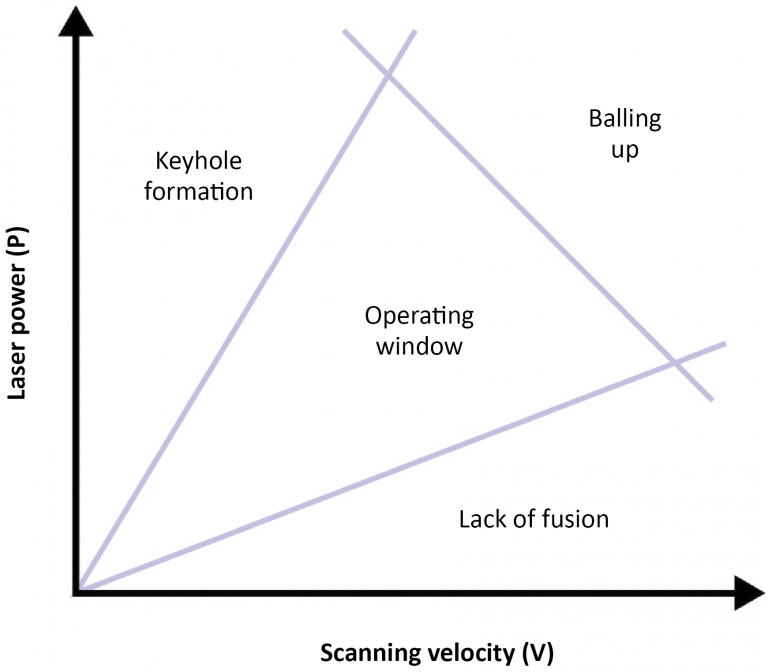
\includegraphics[width=0.6\textwidth]{chapter/main/single/img/scheme_graph.png}
			\caption{Schematische Darstelllung der durch Laserleistung und Lasergeschwindigkeit
			gemeinsamen Wirkung \cite{metalam2018how}}
			\label{fig:sceme_graph}
		\end{figure}

		Abbildung \ref{fig:sceme_graph} zeigt schematisch wie die Lasergeschwindigkeit und
		die Laserleistung zusammen welche Defekte begünstigen und in welchen Bereich an
		Parameterpaaren das Resultat als gut gilt. Anhand der Variation in der Simulation
		können solche Zusammenhänge auf Teilchenebene bestätigt und deshalb besser verstanden
		werden.

		Bevor ein solcher Zusammenhang jedoch konkret erforscht werden kann, bedarf es erstmal
		einer Kalibrierung des Modell beziehungsweise einer Menge an gewählten Startwerten für die
		Parameter, deren Resultate dann als Bezugspunkte innerhalb des Modells dienen. Zu diesem
		Zweck wurde der Einfluss einer Laserleistung bei einer frei gewählten obligatorischen
		Lasergeschwindigkeit von \SI{10}{\angstrom} pro IMD-Zeiteinheit auf die Probe untersucht,
		mit dem Ziel eine Referenzsimulation zu kreieren, deren Rechenzeit vertretbar ist. Dieser
		Punkt ist besonders wichtig, da nach der Einwirkung des Lasers noch ein vielfaches der
		Zeit für die Relaxierung zum neuen Equilibrium aufgewendet werden muss. Von dieser
		Referenzsimulation aus können dann im weiteren Verlauf die einzelnen Parameter variiert
		werden, um deren direkten Einfluss zu untersuchen.

		Als Maß für den geschmolzenen Anteil der Kugel wird eine \emph{Common Neighbor Analysis}
		(\emph{CNA}) verwendet. Eine CNA ist dabei ein Hilfsmittel zur Erkennung und Benennung
		von Gitterstrukturen. Wenn also ein Atom im Aluminium, das bekanntermaßen eine
		fcc-Gitterstruktur hat, als Teil einer anderen Struktur erkannt wird, muss es sich
		zwangsläufig um fluides Aluminium - also die Schmelze - handeln. Dies ist im Großen und
		Ganzen erfahrungsgemäß funktional, jedoch darf nicht vergessen werden, dass Randatome
		(beispielsweise auf Oberflächen) aus geometrischen Gründen falsch erkannt werden können.

		\begin{figure}[!ht]
			\centering
			\begin{subfigure}{0.49\textwidth}
				\centering
				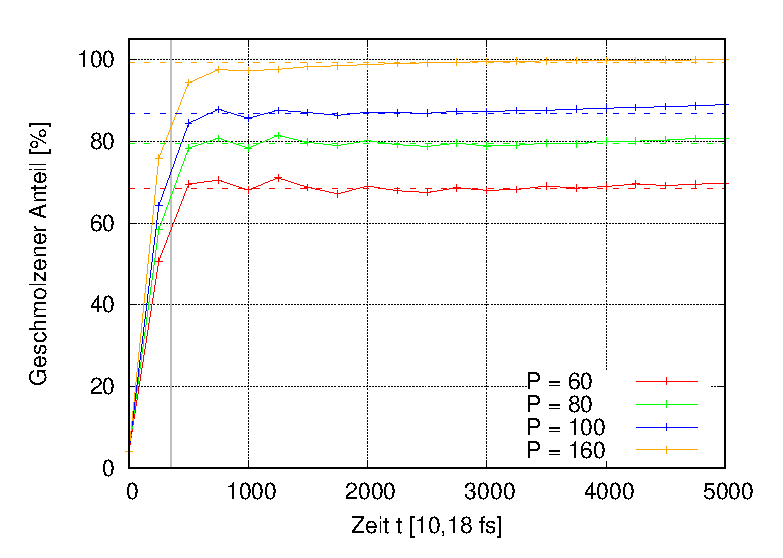
\includegraphics[width=\textwidth]{chapter/main/single/plt/power_calibration/cna_vel10_start.eps}
				\subcaption{Anfangsbereich}
				\label{fig:cna_vel10_start}
			\end{subfigure}
			\begin{subfigure}{0.49\textwidth}
				\centering
				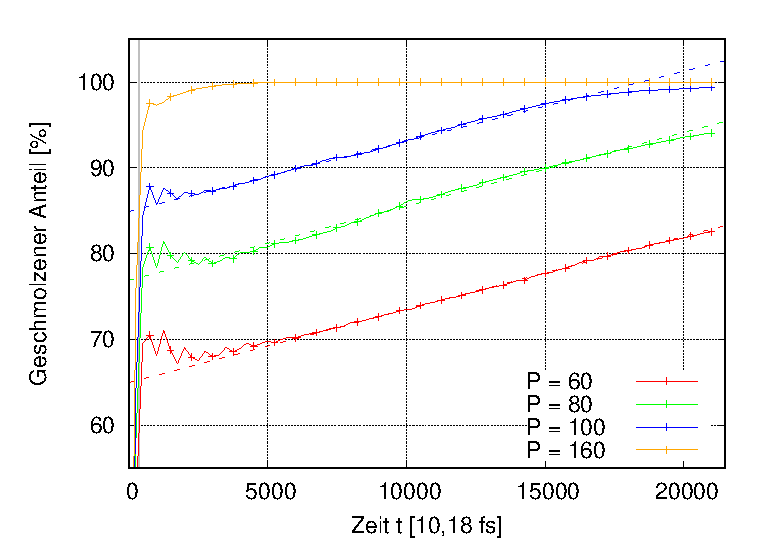
\includegraphics[width=\textwidth]{chapter/main/single/plt/power_calibration/cna_vel10_rate.eps}
				\subcaption{Langzeitentwicklung}
				\label{fig:cna_vel10_rate}
			\end{subfigure}
			\caption{Anteil der Teilchen, die zum geschmolzenen Material zählen über die
			Simulationszeit. Der senkrechte graue Balken markiert den Zeitpunkt zu dem der Laser
			bereits mit Geschwindigkeit $v_\text{Laser} = \SI{10}{\angstrom}$ pro IMD-Zeiteinheit
			vollständig über die Probe gefahren ist.}
			\label{fig:cna_vel10}
		\end{figure}

		In Abbildung \ref{fig:cna_vel10} ist der Anteil des geschmolzenen Materials für
		verschiedene Laserleistungen $P$ über die Zeit aufgetragen. In Abbildung
		\ref{fig:cna_vel10_start} ist der Zeitbereich um den direkten Lasereinfluss vergrößert.
		Hier ist zu sehen, dass der Laser die Probe schlagartig aufschmilzt und der Anteil an
		geschmolzenen Material kurzzeitig konstant bleibt. Durch anfitten eines konstanten Wertes
		in diesem Bereich kann der Anteil an durch die jeweilige Leistung geschmolzenen Materials
		bestimmt werden.

		\begin{table}[!ht]
			\centering
			\caption{Anteil des Materials einer ursprünglich großen Kugel,
			der geschmolzen wird}
			\begin{tabular}{l | r | r}
				Leistung $P$ $\left[\powerunit\right]$
					&	Geschmolzen [\%]
					&	Steigerung $\left[\si{\percent\per\timeunit}\right]$
					\\\hline
				60	&	\SI{68.54}{\percent}	&	0.00085	\\
				80	&	\SI{79.49}{\percent}	&	0.00086	\\
				100	&	\SI{86.95}{\percent}	&	0.00082	\\
				160	&	\SI{99.26}{\percent}	&	0.00084
			\end{tabular}
			\label{tab:vel10_start}
		\end{table}

		Quantifiziert durch Tabelle \ref{tab:vel10_start} ist gut zu erkenen, dass bei einer
		Leistung $P = \powerunit[160]$ die Kugel komplett geschmolzen wird. Der
		fehlende Anteil von $\approx \SI{0.8}{\percent}$ geht auf die Fluktuationen am Anfang
		zurück. In Abbildung \ref{fig:cna_vel10_start} ist schließlich gut zu erkennen, dass der
		Wert die \SI{100}{\percent} noch erreicht.

		Dass die Aufschmelzung vollständig erfolgte, lässt auch Abbildung \ref{fig:vel10_p160}
		vermuten. Der Übersicht wegen wurden hier kleine noch in der Luft auffindbare Spritzer
		mithilfe einer Clusteranalyse identifiziert und ausgeblendet. Für die Bestimmung des
		Schmelzgrades werden diese allerdings berücksichtigt. In der Seitenansich in Abbildung
		\ref{fig:vel10_p160_side} ist auch zu sehen, dass die Schmelze den Untergrund flach und
		breit benetzt. Dies ist auch so in der Realität der Fall \cite{eskandarisabzi2019defect}
		und spricht dafür, dass das Modell mindestens aspekteweise anwendbar ist. Im Großen und
		Ganzen gibt es - augenscheinlich zumindest - auch keine bevorzugte Spritzrichtung
		(Abbildung \ref{fig:vel10_p160_perspective}).

		\begin{figure}[!ht]
			\centering
			\begin{subfigure}{0.5\textwidth}
				\centering
				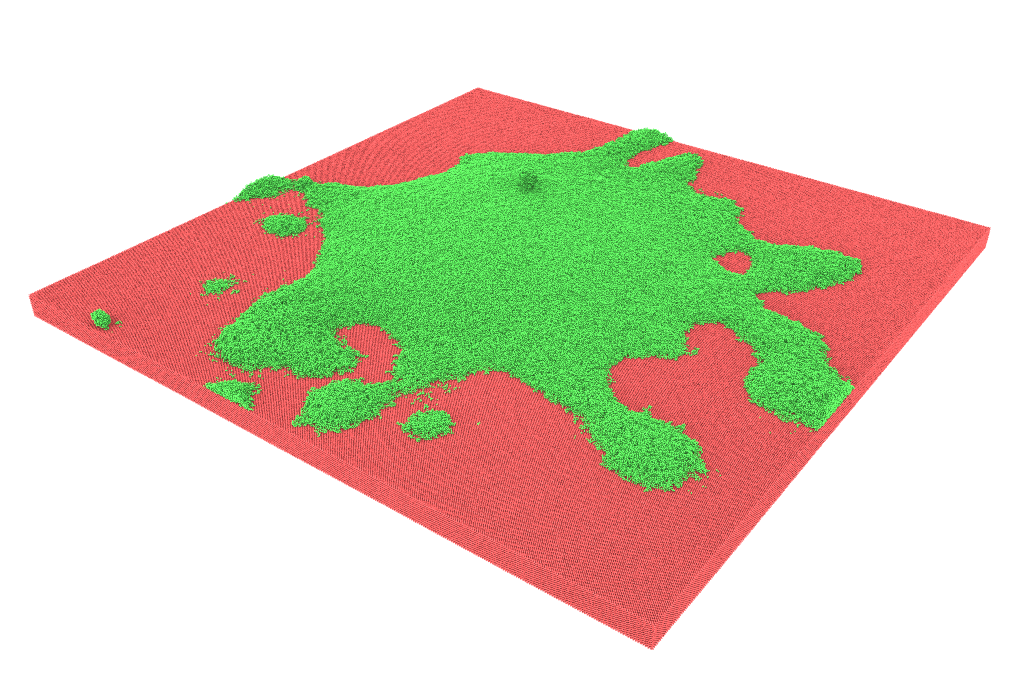
\includegraphics[width=\textwidth]{chapter/main/single/img/power_calibration/v10_p160_c420_perspective.png}
				\subcaption{Perspektivische Ansicht}
				\label{fig:vel10_p160_perspective}
			\end{subfigure}
			\begin{subfigure}{0.9\textwidth}
				\centering
				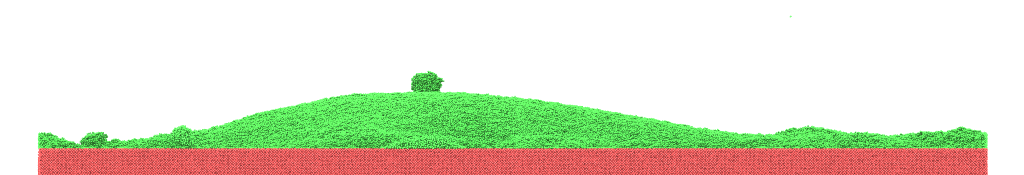
\includegraphics[width=\textwidth]{chapter/main/single/img/power_calibration/v10_p160_c420_side_cropped.png}
				\subcaption{Seitenansicht}
				\label{fig:vel10_p160_side}
			\end{subfigure}
			\caption{Die vollständig aufgeschmolzene Kugel für einen Laser mit
			$P = 160$ Leistungseinheiten nach 21000 IMD-Zeiteinheiten}
			\label{fig:vel10_p160}
		\end{figure}

		Ein interessantes, aber auf den ersten Blick unlogisch erscheinendes, Phänomen ist in
		Abbildung \ref{fig:cna_vel10_rate} für niedrigere Leistungen zu sehen. Während der Anteil
		geschmolzenem Material direkt nach der Lasereinwirkung unter Berücksichtigung hoher
		Fluktuationen konstant ist, ist für längere Zeiträume ein nahezu linearer Anstieg des
		Anteils geschmolzenen Materials zu sehen, bis ein Sättigungseffekt einsetzt. Die
		Steigerungsrate im lineare angenommenen Bereich beträgt für alle Leistungen ungefähr
		gleich viel. Im Schnitt liegt sie bei \SI{8.4e-4}{\percent\per\timeunit} . Dieses
		Verhalten lässt sich leicht erklären. Wenn der Laser einen Teil der Kugel verflüssigt,
		überträgt dieser Teil seine überschüssige Wärme gemäß dem zweiten Hauptsatz der
		Thermodynamik auf den noch ungeschmolzenen Anteil. Ist diese gleichmäßig verteilte Wärme
		groß genug, schmilzt der noch erhärtete Teil ebenfalls. In der Realität ist das
		SLM-Verfahren jedoch kein isoliertes System im thermodynamischen Sinne. Eher das Gegenteil
		ist der Fall: Eine richtige Kühlung ist essentiell für das Verfahren. Wie in Abschnitt
		\ref{subsec:defects} bereits erwähnt kann zu frühes Erstarren zur Poren- oder Rissbildung
		führen, während zu spätes Erstarren ein Stück weit einen Verlust der Mikrostruktur und
		damit der Produktionsgenauigkeit bedeutet \cite{sercombe2016selective}. Gezielt
		eingesetzte Kühlung ist also von fundamentaler Bedeutung.

		\begin{figure}[!ht]
			\centering
			\begin{subfigure}{0.49\textwidth}
				\centering
				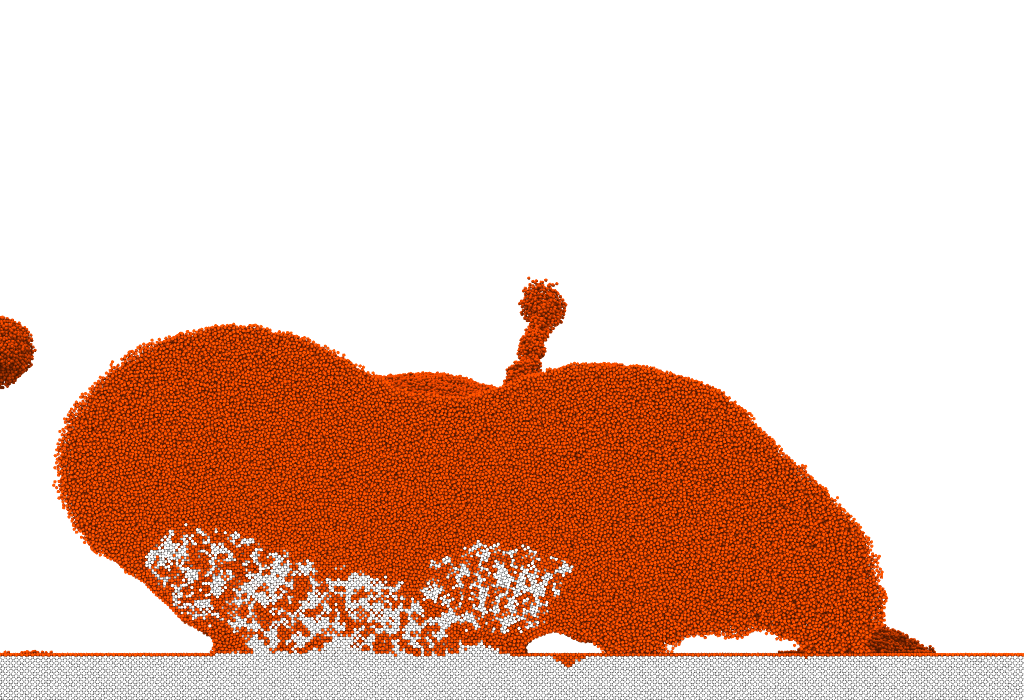
\includegraphics[width=\textwidth]{chapter/main/single/img/power_calibration/v10_p100_c225.png}
				\subcaption{$t = \SI{11250}{\cdot\timeunit}$}
				\label{fig:vel10_p100_earlier}
			\end{subfigure}
			\begin{subfigure}{0.49\textwidth}
				\centering
				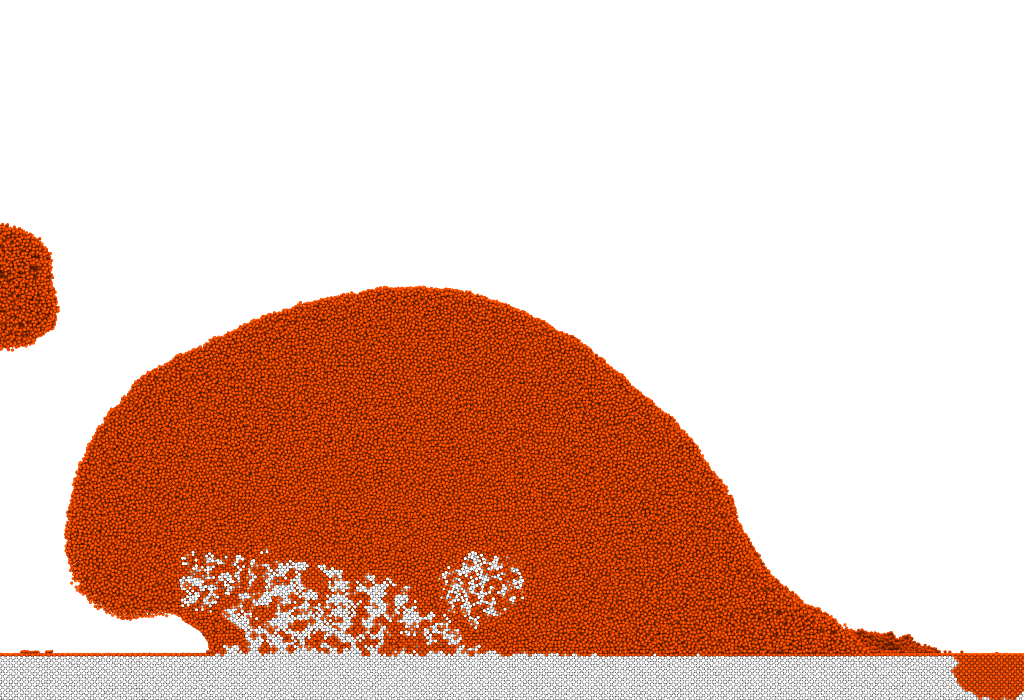
\includegraphics[width=\textwidth]{chapter/main/single/img/power_calibration/v10_p100_c280.png}
				\subcaption{$t = \SI{14000}{\cdot\timeunit}$}
				\label{fig:vel10_p100_later}
			\end{subfigure}
			\caption{Hohlräume verschwinden wegen dem die Probe umgebenden Vakuum. Mit einem
			Schutzgas gefüllt wären die Hohlräume gefüllt und daraus resultierende Defekte wären
			beobachtbar.}
			\label{fig:vel10_p100}
		\end{figure}

		Eine weitere dem Modell geschuldete Ungenauigkeit ist in Abbildung \ref{fig:vel10_p100}
		zu sehen. Es handelt sich um einen Querschnitt durch die Mitte der Kugel in der
		$z$-$x$-Ebene. Rote Atome sind Teil des geschmolzenen Materials, während weiße Atome Teil
		von fcc-Gitterstrukturen sind. Die Kugel wird für $P = 100$ Leistungseinheiten nicht
		vollständig geschmolzen, auch wenn der im vorherigen Abschnitt erläuterte Sachverhalt das
		ungeschmolzene Material nachträglich verschmelzen lässt. Das sieht man besondern gut
		daran, dass der ungeschmolzene Rest mit der Zeit schrumpt. Was an dieser Simulation
		allerdings besonders interessant ist, ist die Tatsache, dass im linken Bild
		Hohlraumbildung zu beobachten ist. Die obere, flüssige Hälfte spritzt seitlich herunter,
		wobei eine flache Ausbreitung wie in Abbildung \ref{fig:vel10_p160} durch den teilweise
		ungeschmolzenen Kern verhindert wird. Die teilweise festen Strukturen führen hier also zur
		Bildung von Hohlräumen. Wie in Abschnitt \ref{subsec:defects} erläutert nennt man die
		dadurch entstandenen Defekte ''Poren''. Leider ist ein paar Simulationsschritte später
		keine Spur der Hohlräume mehr aufzufinden. Das liegt daran, dass Poren eben durch
		Gaseinschlüsse entstehen. Da in der hier betrachteten Simulation die Probe jedoch von
		einem Vakuum umgeben ist, konnte umliegendes Material einfach den Hohlraum eindringen
		und die Pore so schließen.


\section{Verhalten bei halbierter Lasergeschwindigkeit}
		Nachdem jetzt ein Methode zur Übertragung der Simulationsergebnisse auf experimentelle
		Daten bekannt ist
